\documentclass{beamer}
\usepackage{tikz,amsmath,hyperref,graphicx,stackrel,animate,tipa}
\usetikzlibrary{positioning,shadows,arrows,shapes,calc}
\newcommand{\ipa}[1]{\textipa{#1}}
\newcommand{\argmax}{\operatornamewithlimits{argmax}}
\newcommand{\argmin}{\operatornamewithlimits{argmin}}
\mode<presentation>{\usetheme{Frankfurt}}
\DeclareMathOperator*{\softmax}{softmax}
\AtBeginSection[]
{
  \begin{frame}<beamer>
    \frametitle{Outline}
    \tableofcontents[currentsection,currentsubsection]
  \end{frame}
}
\title{Lecture 13: How to train Observation Probability Densities}
\author{Mark Hasegawa-Johnson\\All content~\href{https://creativecommons.org/licenses/by-sa/4.0/}{CC-SA 4.0} unless otherwise specified.}
\date{ECE 417: Multimedia Signal Processing, Fall 2020}  
\begin{document}

% Title
\begin{frame}
  \maketitle
\end{frame}

% Title
\begin{frame}
  \tableofcontents
\end{frame}

%%%%%%%%%%%%%%%%%%%%%%%%%%%%%%%%%%%%%%%%%%%%
\section[Review]{Review: Hidden Markov Models}
\setcounter{subsection}{1}

\begin{frame}
  \frametitle{Hidden Markov Model}

  \begin{center}
    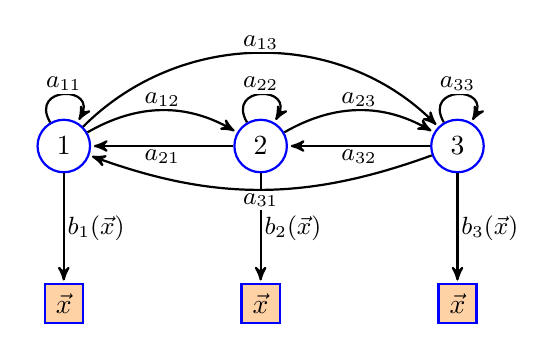
\begin{tikzpicture}[->,>=stealth',shorten >=1pt,auto,node distance=3cm,thick,
        state/.style={circle,thick,draw=blue,text=black,text centered,text width=0.25cm},
        obs/.style={rectangle,thick,draw=blue,text=black,fill=orange!35!white,text centered,text width=0.25cm}
      ]
      \node[state] (q1) at (0,0) {1};
      \node[state] (q2) at (2.5,0) {2};
      \node[state] (q3) at (5,0) {3};
      \node[obs] (x1) at (0,-2) {$\vec{x}$};
      \node[obs] (x2) at (2.5,-2) {$\vec{x}$};
      \node[obs] (x3) at (5,-2) {$\vec{x}$};
      \path[every node/.style={font=\sffamily\small,
  	  fill=white,inner sep=1pt}]
      (q1) edge [out=120,in=60,looseness=4] node {$a_{11}$} (q1)
      edge [out=30,in=150] node {$a_{12}$} (q2)
      edge [out=45,in=135] node {$a_{13}$} (q3)
      edge [out=-90,in=90] node {$b_1(\vec{x})$} (x1)
      (q2) edge [out=120,in=60,looseness=4] node {$a_{22}$} (q2)
      edge [out=180,in=0] node {$a_{21}$} (q1)
      edge [out=30,in=150] node {$a_{23}$} (q3)
      edge [out=-90,in=90] node {$b_2(\vec{x})$} (x2)
      (q3) edge [out=120,in=60,looseness=4] node {$a_{33}$} (q3)
      edge [out=180,in=0] node {$a_{32}$} (q2)
      edge [out=-160,in=-20] node {$a_{31}$} (q1)
      edge [out=-90,in=90] node {$b_3(\vec{x})$} (x3);
    \end{tikzpicture}
  \end{center}
  \begin{enumerate}
  \item Start in state $q_t=i$ with pmf $\pi_i$.
  \item Generate an observation, $\vec{x}$, with pdf $b_i(\vec{x})$.
  \item Transition to a new state, $q_{t+1}=j$, according to pmf $a_{ij}$.
  \item Repeat.
  \end{enumerate}
\end{frame}

\begin{frame}
  \frametitle{The Forward Algorithm}

  Definition: $\alpha_t(i) \equiv p(\vec{x}_1,\ldots,\vec{x}_t,q_t=i|\Lambda)$.  Computation:
  \begin{enumerate}
  \item {\bf Initialize:}
    \[
    \alpha_1(i) = \pi_i b_i(\vec{x}_1),~~~1\le i\le N
    \]
  \item {\bf Iterate:}
    \begin{align*}
      \alpha_{t}(j) &= \sum_{i=1}^N \alpha_{t-1}(i) a_{ij}b_j(\vec{x}_t),~~1\le j\le N,~2\le t\le T
    \end{align*}
  \item {\bf Terminate:}
    \[
    p(X|\Lambda) = \sum_{i=1}^N \alpha_T(i)
    \]
  \end{enumerate}
\end{frame}
  
\begin{frame}
  \frametitle{The Backward Algorithm}

  Definition: $\beta_t(i) \equiv p(\vec{x}_{t+1},\ldots,\vec{x}_T|q_t=i,\Lambda)$.  Computation:
  \begin{enumerate}
  \item {\bf Initialize:}
    \[
    \beta_T(i) = 1,~~~1\le i\le N
    \]
  \item {\bf Iterate:}
    \begin{align*}
      \beta_{t}(i) &= \sum_{j=1}^N a_{ij}b_j(\vec{x}_{t+1})\beta_{t+1}(j),~~1\le i\le N,~1\le t\le T-1
    \end{align*}
  \item {\bf Terminate:}
    \[
    p(X|\Lambda) = \sum_{i=1}^N \pi_ib_i(\vec{x}_1)\beta_1(i)
    \]
  \end{enumerate}
\end{frame}

\begin{frame}
  \frametitle{The Baum-Welch Algorithm}

  \begin{enumerate}
  \item {\bf Initial State Probabilities:}
    \begin{align*}
      \pi_i' &=\frac{\sum_{sequences} \gamma_1(i)}{\mbox{\# sequences}}
    \end{align*}
  \item {\bf Transition Probabilities:}
    \begin{align*}
      a_{ij}' &=\frac{\sum_{t=1}^{T-1} \xi_t(i,j)}{\sum_{j=1}^N\sum_{t=1}^{T-1}\xi_t(i,j)}
    \end{align*}
  \item {\bf Observation Probabilities:} 
    \begin{align*}
      {\mathcal L} &= -\frac{1}{T}\sum_{t=1}^T\sum_{i=1}^N  \gamma_t(i)\ln b_{i}(\vec{x}_t)
    \end{align*}
  \end{enumerate}
\end{frame}

%%%%%%%%%%%%%%%%%%%%%%%%%%%%%%%%%%%%%%%%%%%%
\section[Softmax]{Softmax Observation Probabilities}
\setcounter{subsection}{1}

\begin{frame}
  \frametitle{Review: Conditional Probability}

  The relationship among posterior, prior, evidence and likelihood is
  \begin{displaymath}
    p(q|\vec{x})p(\vec{x})=p(\vec{x}|q)p(q)
  \end{displaymath}
  Since softmax is normalized so that $1=\sum_q \softmax(e[q])$, it
  makes most sense to interpret $\softmax(e[q])=p(q|\vec{x})$.
  Therefore, the likelihood should be
  \begin{displaymath}
    b_q(\vec{x}) \equiv p(\vec{x}|q) = \frac{p(\vec{x})\softmax(e[q])}{p(q)}
  \end{displaymath}
\end{frame}
  
\begin{frame}
  \frametitle{Relationship between the likelihood and the posterior}
  
  Therefore, the likelihood should be
  \begin{displaymath}
    b_q(\vec{x}) \equiv p(\vec{x}|q) = \frac{p(\vec{x})\softmax(e[q])}{p(q)}
  \end{displaymath}
  However,
  \begin{itemize}
  \item If we choose training data with equal numbers of each phone, then
    we can assume $p(q)=1/N$.
  \item $p(\vec{x})$ is independent of $q$, so it doesn't affect
    recognition.  So let's assume that  $p(\vec{x})=1/N$ also.
  \end{itemize}
\end{frame}
  
\begin{frame}
  \frametitle{Softmax Observation Probabilities}

  Given the assumptions that $p(q)=p(\vec{x})=1/N$, 
  \begin{displaymath}
    b_q(\vec{x}) = p(\vec{x}|q)=p(q|\vec{x}) = \softmax(e[q])
  \end{displaymath}
  The assumptions are unrealistic.  We sometimes need to adjust for
  low-frequency phones, in order to get good-quality recognition.  But
  let's first derive the solution given these assumptions, and then
  we'll see if the assumptions can be relaxed.
\end{frame}

\begin{frame}
  \frametitle{Softmax Observation Probabilities}

  Given the assumptions that $p(q)=p(\vec{x})=1/N$, 
  \begin{displaymath}
    b_q(\vec{x}) = \softmax(e[q]) = \frac{\exp(e[q])}{\sum_{\ell=1}^N \exp(e[\ell])},
  \end{displaymath}
  where $e[i]$ is the $i^{\textrm{th}}$ element of the output
  excitation row vector, $\vec{e}=\vec{h}W$, computed as the product of a
  weight matrix $W$ with the hidden layer activation row vector, $\vec{h}$.
\end{frame}

\begin{frame}
  \frametitle{Expected negative log likelihood}

  The neural net is trained to minimize the expected negative log
  likelihood, a.k.a. the cross-entropy between $\gamma_t(i)$ and
  $b_i(\vec{x}_t)$:
  \begin{displaymath}
    {\mathcal L}_{CE} = -\frac{1}{T}\sum_{t=1}^T\sum_{i=1}^N\gamma_t(i)\ln b_i(\vec{x}_t)
  \end{displaymath}
  Remember that, since $\vec{e}=\vec{h}W$, the weight gradient is just:
  \begin{displaymath}
    \frac{d{\mathcal L}_{CE}}{dw_{jk}} =
    \sum_{t=1}^T \frac{d{\mathcal L}_{CE}}{de_t[k]}\frac{\partial e_t[k]}{\partial w_{jk}}
    = \sum_{t=1}^T\frac{d{\mathcal L}_{CE}}{de_t[k]}h_t[j],
  \end{displaymath}
  where $h_t[j]$ is the $j^{\textrm{th}}$ component of $\vec{h}$ at time $t$, and
  $e_t[k]$ is the $k^{\textrm{th}}$ component of $\vec{e}$ at time $t$.
\end{frame}

\begin{frame}
  \frametitle{Back-prop}

  Let's find the loss gradient w.r.t. $e_t[k]$.
  The loss is
  \begin{displaymath}
    {\mathcal L}_{CE} = -\frac{1}{T}\sum_{t=1}^T\sum_{i=1}^N\gamma_t(i)\ln b_i(\vec{x}_t)
  \end{displaymath}
  so its gradient is
  \begin{displaymath}
    \frac{d{\mathcal L}_{CE}}{de_t[k]} = -\frac{1}{T}\sum_{i=1}^N\frac{\gamma_t(i)}{b_i(\vec{x}_t)}\frac{\partial b_i(\vec{x}_t)}{\partial e_t[k]}
  \end{displaymath}
\end{frame}

\begin{frame}
  \frametitle{Differentiating the softmax}

  The softmax is
  \begin{displaymath}
    b_i(\vec{x}) =\frac{\exp(e[i])}{\sum_\ell \exp(e[\ell])}=\frac{A}{B}
  \end{displaymath}
  Its  derivative is
  \begin{align*}
    \frac{\partial b_i(\vec{x})}{\partial e[k]}
    &= \frac{1}{B}\frac{\partial A}{\partial e[k]}-\frac{A}{B^2}\frac{\partial B}{\partial e[k]}\\
    &=\begin{cases}
    \frac{\exp(e[i])}{\sum_\ell\exp(e[\ell])}-
    \frac{\exp(e[i])^2}{\left(\sum_\ell\exp(e[\ell])\right)^2} & i=k\\
    -\frac{\exp(e[i])\exp(e[k])}{\left(\sum_\ell\exp(e[\ell])\right)^2} & i\ne k
    \end{cases}\\
    &=\begin{cases}
    b_i(\vec{x})-b_i^2(\vec{x}) & i=k\\
    -b_i(\vec{x})b_k(\vec{x}) &  i\ne k
    \end{cases}
  \end{align*}
\end{frame}

\begin{frame}
  \frametitle{The loss gradient}

  The loss gradient it
  \begin{align*}
    \frac{d{\mathcal L}_{CE}}{de_t[k]}
    &= -\frac{1}{T}\sum_{i=1}^N\frac{\gamma_t(i)}{b_i(\vec{x}_t)}\frac{\partial b_i(\vec{x}_t)}{\partial e_t[k]}\\
    &= -\frac{1}{T}\left(\gamma_t(k)(1-b_k(\vec{x}_t))-\sum_{i\ne k}\gamma_t(i)b_k(t)\right)\\
    &= -\frac{1}{T}\left(\gamma_t(k)-b_k(\vec{x}_t)\sum_{i=1}^N\gamma_t(i)\right)\\
    &= -\frac{1}{T}\left(\gamma_t(k)-b_k(\vec{x}_t)\right)
  \end{align*}
\end{frame}

\begin{frame}
  \frametitle{Summary: softmax observation probabilities}

  Training $W$ to minimize the cross-entropy  between $\gamma_t(i)$ and $b_i(t)$,
  \begin{displaymath}
    {\mathcal L}_{CE} = -\frac{1}{T}\sum_{t=1}^T\sum_{i=1}^N\gamma_t(i)\ln b_i(\vec{x}_t),
  \end{displaymath}
  yields the following weight gradient:
  \begin{displaymath}
    \frac{d{\mathcal L}_{CE}}{dw_{jk}}=
    -\frac{1}{T}\sum_{t=1}^T h_{t}[j]\left(\gamma_t(k)-b_k(\vec{x}_t)\right)
  \end{displaymath}
  which vanishes when the neural net estimates
  $b_k(\vec{x}_t)\rightarrow \gamma_t(k)$ as well as it can.
\end{frame}

\begin{frame}
  \frametitle{Summary: softmax observation probabilities}

  The Baum-Welch algorithm alternates between two types of estimation,
  often called the E-step (expectation) and the M-step (maximization
  or minimization):
  \begin{enumerate}
  \item {\bf E-step:} Use forward-backward algorithm to re-estimate
    $\gamma_t(i)=p(q_t=i|X,\Lambda)$.
  \item {\bf M-step:} Train the neural net for a few iterations of
    gradient descent, so that $b_k(\vec{x}_t)\rightarrow \gamma_t(k)$.
  \end{enumerate}
\end{frame}

\begin{frame}
  \frametitle{Final note: Those ridiculous assumptions}

  As a final note, let's see if we can eliminate those ridiculous
  assumptions, $p(q)=p(\vec{x})=1/N$.  {\bf How?}  Well, the weight
  gradient goes to zero when $\sum_{t=1}^T
  h_{t}[j]\left(\gamma_t(k)-b_k(\vec{x}_t)\right)=0$.  There are at
  least two ways in which this can happen:
  \begin{enumerate}
  \item $b_k(\vec{x}_t)=\gamma_t(k)$.  The neural net is successfully
    estimating the posterior.  This is the best possible solution if
    $p(q=i)=p(\vec{x})=\frac{1}{N}$.
  \item $b_k(\vec{x}_t)-\gamma_t(k)$ is uncorrelated with $h_t[j]$,
    e.g., because it is zero mean and independent of $\vec{x}_t$.
  \end{enumerate}
\end{frame}

\begin{frame}
  \frametitle{Final note: Those ridiculous assumptions}

  The weight gradient goes to zero if $\gamma_t(k)-b_k(\vec{x}_t)$ is
  zero mean and independent of $\vec{x}_t$.  For example,
  \begin{itemize}
  \item $b_k(\vec{x})$ might differ from $\gamma_t(k)$ by a global
    scale factor.  Instead of softmax, we might use some other
    normalization, either because (a) it's scaled more like a
    likelihood, or (b) it has nice numerical properties.  An example
    of (b) is:
    \[
    b_i(\vec{x}) = \frac{\exp(e[i])}{\max_j \exp(e[j])}
    \]
  \item $b_k(\vec{x})$ might differ from $\gamma_t(k)$ by a
    phone-dependent scale factor, e.g., we might choose
    \[
    b_i(\vec{x}) =\frac{p(q=i|\vec{x})}{p(q=i)}=
    \frac{\exp(e[i])}{p(q=i)\sum_{j=1}^N\exp(e[j])}
    \]
  \end{itemize}
\end{frame}


%%%%%%%%%%%%%%%%%%%%%%%%%%%%%%%%%%%%%%%%%%%%
\section[Gaussians]{Gaussian Observation Probabilities}
\setcounter{subsection}{1}

\begin{frame}
  \frametitle{Baum-Welch with Gaussian Probabilities}

  Baum-Welch asks us to minimize the cross-entropy between
  $\gamma_t(i)$ and $b_i(\vec{x}_t)$:
  \begin{displaymath}
    {\mathcal L}_{CE} = -\frac{1}{T}\sum_{t=1}^T\sum_{i=1}^N\gamma_t(i)\ln b_i(\vec{x}_t)
  \end{displaymath}
  In order to force $b_i(\vec{x}_t)$ to be a likelihood, rather than a
  posterior, one way is to use a function that is guaranteed to be a
  properly normalized pdf.  For example, a Gaussian:
  \begin{displaymath}
    b_i(\vec{x}) = {\mathcal N}\left(\vec{x};\vec\mu_i,\Sigma_i\right)
  \end{displaymath}
\end{frame}
  
\begin{frame}
  \frametitle{Diagonal-Covariance Gaussian pdf}

  Let's assume the feature vector has $D$ dimensions,
  $\vec{x}=[x_1,\ldots,x_D]$.  The Gaussian pdf is
  \begin{displaymath}
    {\mathcal N}\left(\vec{x};\vec\mu,\Sigma\right)=
    \frac{1}{(2\pi)^{D/2}|\Sigma|^{1/2}}e^{-\frac{1}{2}(\vec{x}-\vec\mu)\Sigma^{-1}(\vec{x}-\vec\mu)^T}
  \end{displaymath}
  Let's assume a diagonal covariance matrix,
  $\Sigma=\mbox{diag}(\sigma_1^2,\ldots,\sigma_D^2)$, so that
  \begin{displaymath}
    {\mathcal N}\left(\vec{x};\vec\mu,\Sigma\right)=
    \frac{1}{\sqrt{\prod_{d=1}^D2\pi\sigma_d^2}}e^{-\frac{1}{2}\sum_{d=1}^D\frac{(x_d-\mu_d)^2}{\sigma_d^2}}
  \end{displaymath}
\end{frame}
  
\begin{frame}
  \frametitle{Logarithm of a diagonal covariance Gaussian}

  The logarithm of a diagonal-covariance Gaussian is
  \begin{displaymath}
    \ln b_i(\vec{x})=
    -\frac{1}{2}\sum_{d=1}^D\frac{(x_d-\mu_d)^2}{\sigma_d^2}
    -\frac{1}{2}\sum_{d=1}^D\ln\sigma_d^2
    -\frac{D}{2}\ln(2\pi)
  \end{displaymath}
\end{frame}

\begin{frame}
  \frametitle{Minimizing the cross-entropy}

  Surprise!  The cross-entropy between $\gamma_t(i)$ and
  $b_i(\vec{x}_t)$ can be minimized in closed form, if $b_i(\vec{x})$
  is Gaussian.
  \begin{align*}
    {\mathcal L}_{CE}
    &= -\frac{1}{T}\sum_{t=1}^T\sum_{i=1}^N\gamma_t(i)\ln b_i(\vec{x}_t)\\
    &= \frac{1}{2T}\sum_{t=1}^T\sum_{i=1}^N\gamma_t(i)\left(
    \sum_{d=1}^D\frac{(x_{td}-\mu_{id})^2}{\sigma_{id}^2}
    +\sum_{d=1}^D\ln\sigma_{id}^2
    +D\ln(2\pi)\right)
  \end{align*}
  It's possible to choose $\mu_{id}$ and $\sigma_{id}^2$ so that
  \begin{displaymath}
    \frac{d{\mathcal L}_{CE}}{d\mu_{qd}}=
    \frac{d{\mathcal L}_{CE}}{d\sigma_{qd}^2}=0
  \end{displaymath}
\end{frame}
  
\begin{frame}
  \frametitle{Minimizing the cross-entropy: optimum $\mu$}

  First, let's optimize $\mu_{id}$.  We want
  \begin{displaymath}
    0 = \frac{d}{d\mu_{qd}}\sum_{t=1}^T\sum_{i=1}^N\gamma_t(i)\left(\sum_{d=1}^D\frac{(x_{td}-\mu_{id})^2}{\sigma_{id}^2}\right)
  \end{displaymath}
  Re-arranging terms, we get
  \begin{displaymath}
    \mu_{qd} = \frac{\sum_{t=1}^T\gamma_t(q)x_{td}}{\sum_{t=1}^T\gamma_t(q)}
  \end{displaymath}
\end{frame}

\begin{frame}
  \frametitle{Minimizing the cross-entropy: optimum $\sigma$}

  Second, let's optimize $\sigma_{id}^2$.  We want
  \begin{displaymath}
    0 = \frac{d}{d\sigma_{qd}^2}\sum_{t=1}^T\sum_{i=1}^N\gamma_t(i)\left(
    \sum_{d=1}^D\frac{(x_{td}-\mu_{id})^2}{\sigma_{id}^2}    +\sum_{d=1}^D\ln\sigma_{id}^2\right)
  \end{displaymath}
  Re-arranging terms, we get
  \begin{displaymath}
    \sigma_{qd}^2 = \frac{\sum_{t=1}^T\gamma_t(q)(x_{td}-\mu_{qd})^2}{\sum_{t=1}^T\gamma_t(q)}
  \end{displaymath}
\end{frame}

\begin{frame}
  \frametitle{Summary: Gaussian observation probabilities}

  A Gaussian pdf can be optimized in closed form.
  \begin{enumerate}
  \item The mean is the weighted average of feature vectors:
    \begin{displaymath}
      \mu_{id} = \frac{\sum_{t=1}^T\gamma_t(i)x_{td}}{\sum_{t=1}^T\gamma_t(i)}
    \end{displaymath}
  \item The variance is the weighted average of squared feature vectors:
    \begin{displaymath}
      \sigma_{id}^2 = \frac{\sum_{t=1}^T\gamma_t(i)(x_{td}-\mu_{id})^2}{\sum_{t=1}^T\gamma_t(i)}
    \end{displaymath}
  \end{enumerate}
  \ldots and then we would re-compute $\gamma_t(i)$ using
  forward-backward, and so on.
\end{frame}

%%%%%%%%%%%%%%%%%%%%%%%%%%%%%%%%%%%%%%%%%%%%
\section[Discrete]{Discrete Observation Probabilities}
\setcounter{subsection}{1}

\begin{frame}
  \frametitle{Baum-Welch with Discrete Probabilities}

  Finally, suppose that $x_t$ is discrete, for example,
  $x_t\in\left\{1,\ldots,K\right\}$.  In this case, a pretty
  reasonable way to model the observations is using a lookup table:
  \begin{displaymath}
  b_i(k)\ge 0,~~~1=\sum_{k=1}^K b_i(k)
  \end{displaymath}
\end{frame}

\begin{frame}
  \frametitle{Optimizing a discrete observation pmf}
  
  Again, Baum-Welch asks us to minimize the
  cross-entropy between $\gamma_t(i)$ and $b_i(x_t)$:
  \begin{displaymath}
    {\mathcal L}_{CE} = -\frac{1}{T}\sum_{t=1}^T\sum_{i=1}^N\gamma_t(i)\ln b_i(x_t),
  \end{displaymath}
  but now we also have this constraint to satisfy:
  \begin{displaymath}
    1=\sum_{k=1}^K b_i(k)
  \end{displaymath}
\end{frame}
  
\begin{frame}
  \frametitle{The Lagrangian}

  We can find the values $b_i(k)$ that minimize ${\mathcal L}_{CE}$
  subject to the constraint using a method called Lagrangian
  optimization.  Basically, we create a {\em Lagrangian}, which is
  defined to be the original criterion plus $\lambda$ times the
  constraint:
  \begin{displaymath}
    {\mathcal L} = -\sum_{t=1}^T\sum_{i=1}^N\gamma_t(i)\ln b_i(x_t)+
    \lambda\left(1-\sum_{k=1}^K b_i(k)\right)
  \end{displaymath}
  The idea is that there are an infinite number of solutions that will
  set $\frac{d{\mathcal L}}{db_q(k)}=0$; we will choose the one that also sets $\sum_k
  b_i(k)=1$.
\end{frame}
  
\begin{frame}
  \frametitle{Differentiating The Lagrangian}

  Differentiating the Lagrangian gives
  \begin{displaymath}
    \frac{d{\mathcal L}}{db_q(k)} = -\sum_{t:x_t=k}\frac{\gamma_t(q)}{b_q(k)}-\lambda
  \end{displaymath}
  Setting $\frac{d{\mathcal L}}{db_q(k)}=0$ gives
  \begin{displaymath}
    b_q(k)=\frac{1}{\lambda}\sum_{t:x_t=k}\gamma_t(q)
  \end{displaymath}
  Then we choose $\lambda$ so that $\sum b_q(k)=1$.
\end{frame}

%%%%%%%%%%%%%%%%%%%%%%%%%%%%%%%%%%%%%%%%%%%%
\section[Summary]{Summary}
\setcounter{subsection}{1}

\begin{frame}
  \frametitle{Summary: Estimating the Observation Probability Densities}

  The Baum-Welch algorithm alternates between two steps, sometimes
  called the E-step (expectation) and the M-step (maximization or
  minimization):
  \begin{enumerate}
  \item {\bf E-step:} Use forward-backward algorithm to re-estimate
    the posterior probability of the hidden state variable,
    $\gamma_t(i)=p(q_t=i|X,\Lambda)$, given the current model
    parameters.
  \item {\bf M-step:} re-estimate the model parameters, in order to
    minimize the cross-entropy between $\gamma_t(i)$ and $b_i(x_t)$:
    \begin{displaymath}
      {\mathcal L}_{CE} = -\frac{1}{T}\sum_{t=1}^T\sum_{i=1}^N\gamma_t(i)\ln b_i(x_t).
    \end{displaymath}
  \end{enumerate}
\end{frame}

\begin{frame}
  \frametitle{Three Types of Observation Probabilities}
  \begin{itemize}
  \item Minimizing ${\mathcal L}_{CE}$ for a softmax gives
    \begin{displaymath}
      \frac{d{\mathcal L}_{CE}}{dw_{jk}}=
      -\frac{1}{T}\sum_{t=1}^T h_{t}[j]\left(\gamma_t(k)-b_k(\vec{x}_t)\right)
    \end{displaymath}
  \item Minimizing ${\mathcal L}_{CE}$ for a Gaussian gives
    \begin{align*}
      \mu_{id} &= \frac{\sum_{t=1}^T\gamma_t(i)x_{td}}{\sum_{t=1}^T\gamma_t(i)}\\
      \sigma_{id}^2 &= \frac{\sum_{t=1}^T\gamma_t(i)(x_{td}-\mu_{id})^2}{\sum_{t=1}^T\gamma_t(i)}
    \end{align*}
  \item Minimizing ${\mathcal L}_{CE}$ for a discrete pmf gives
    \begin{displaymath}
      b_i(k)=\frac{\sum_{t:x_t=k}\gamma_t(i)}{\sum_{t=1}^T \gamma_t(i)}
    \end{displaymath}
  \end{itemize}
\end{frame}

\end{document}

